%%%%%%%%%%%%%%%%%%%%%%%%%%%%%%%%%%%%%%%%%%%%%%%%%%%%%%%%%%%%%%%
%
% Welcome to Overleaf --- just edit your LaTeX on the left,
% and we'll compile it for you on the right. If you open the
% 'Share' menu, you can invite other users to edit at the same
% time. See www.overleaf.com/learn for more info. Enjoy!
%
%%%%%%%%%%%%%%%%%%%%%%%%%%%%%%%%%%%%%%%%%%%%%%%%%%%%%%%%%%%%%%%
\documentclass{beamer}
\usepackage{babel,blindtext}
\usepackage[backend=biber,isbn=false,url=false]{biblatex} 
\addbibresource{refsPres.bib}
\setbeamerfont{footnote}{size=\tiny}
%Information to be included in the title page:
\title{Algorithmic Transit Optimization: Evolutionary Algorithms Applied}
\author{Harrison Weinstock}
\institute{Haverford College}
\date{\today}

\begin{document}

\frame{\titlepage}

\begin{frame}{Designing a System}

\minipage{0.33\textwidth}
  \begin{enumerate}
    \item \textbf{Network geometry}
    \item Frequency Assignment and Timetable Development
    \item Fleet and Crew Scheduling
    \end{enumerate}
\endminipage\hfill
\minipage{0.66\textwidth}%
\begin{figure}
  \fbox{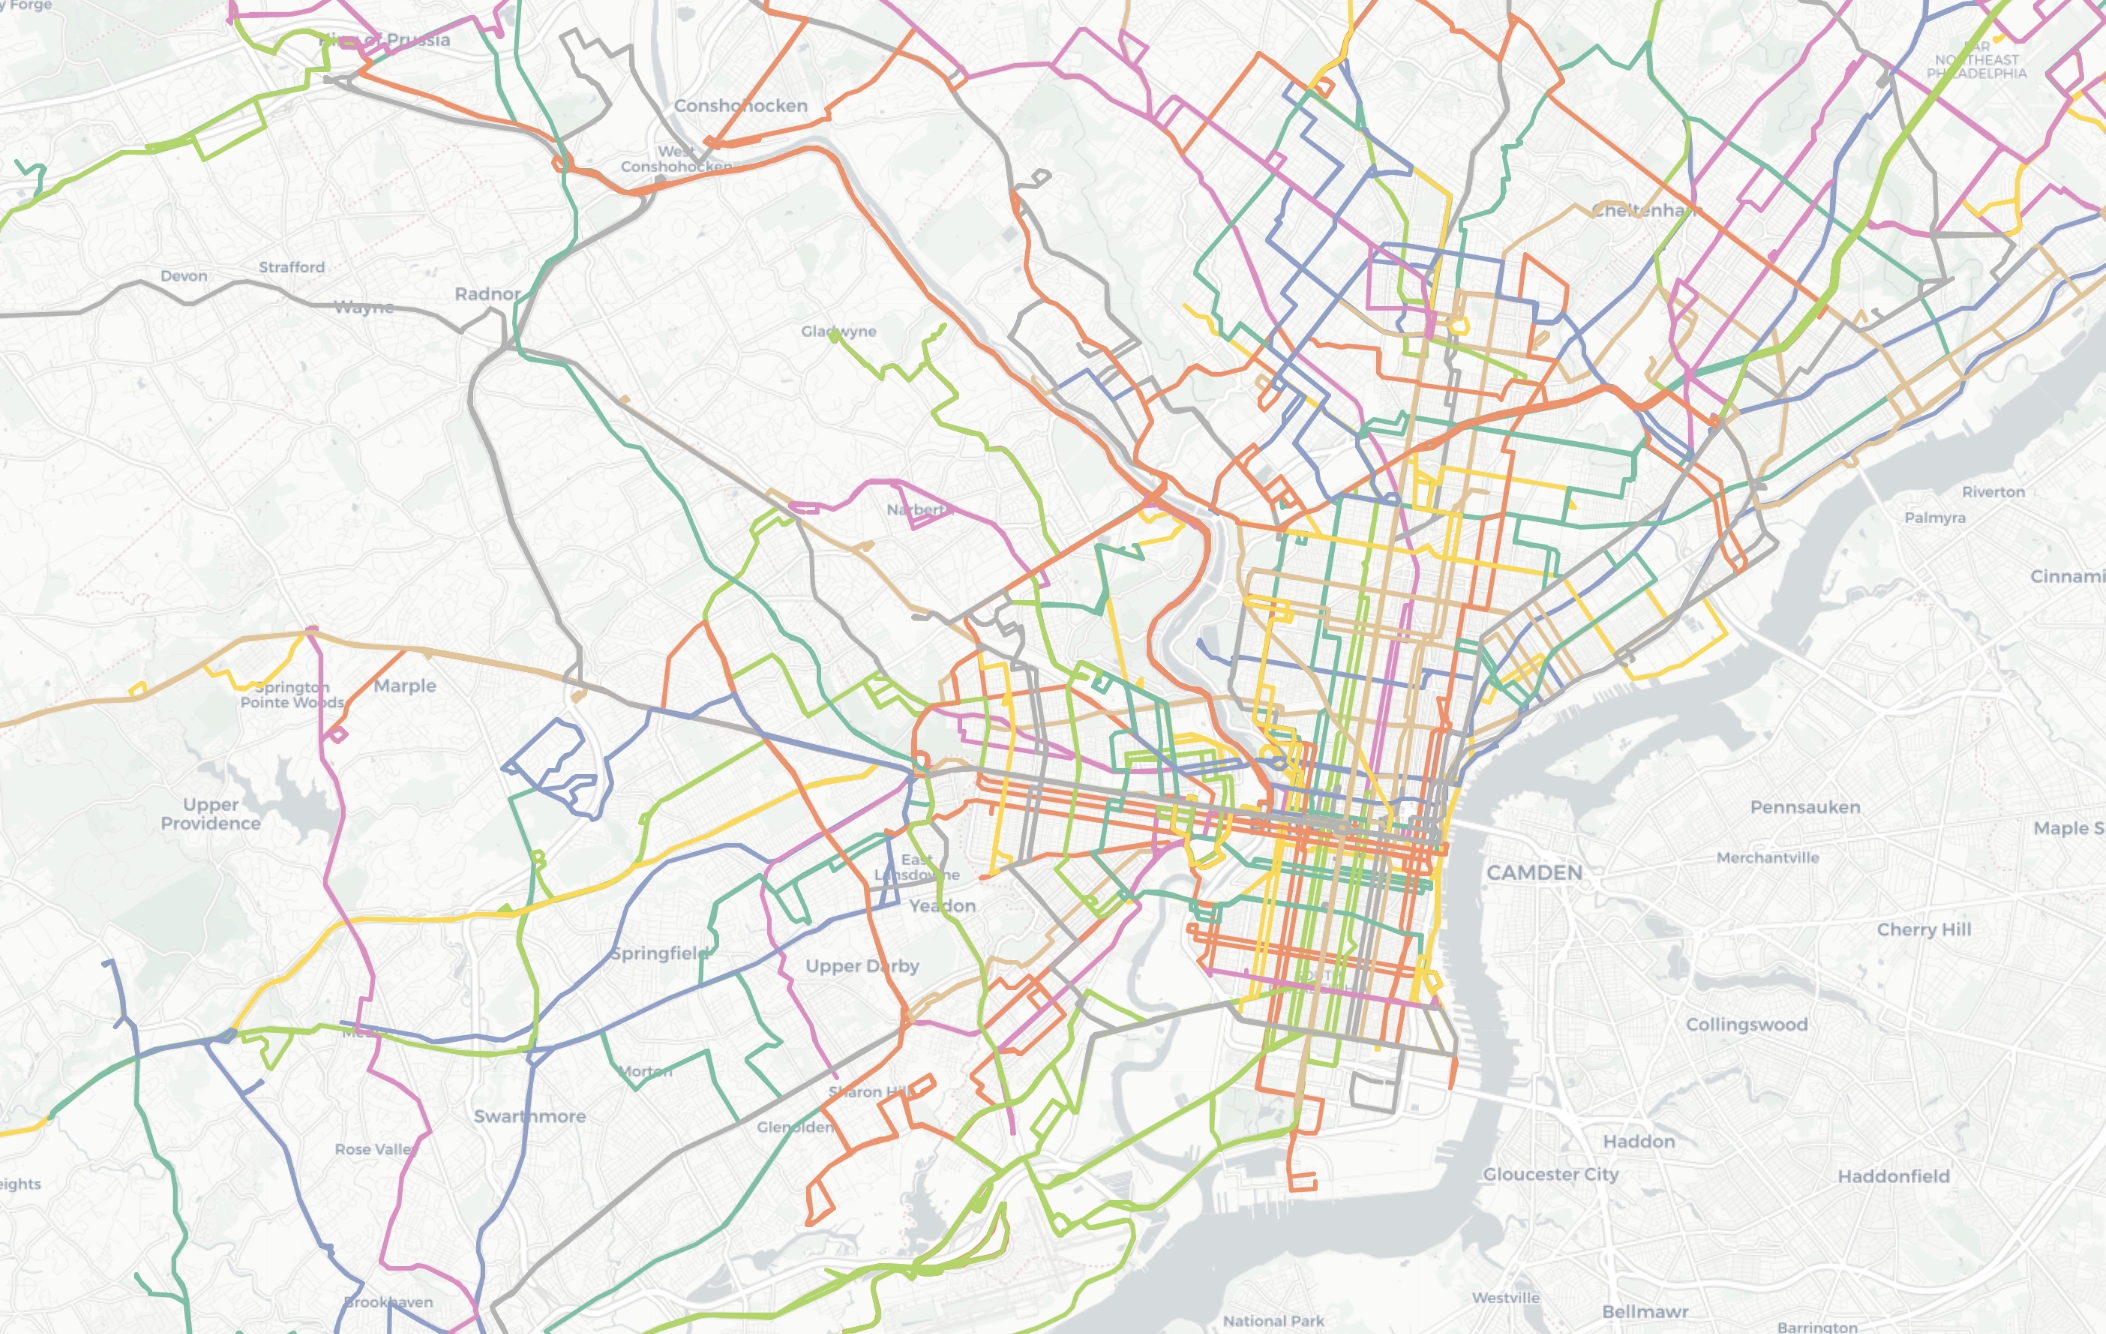
\includegraphics[width=\linewidth]{Presentation/diagrams/septa_screenshot.png}}
  \caption{SEPTA Service around Philadelphia \cite{SEPTA}}
\end{figure}
\endminipage
\end{frame}

\begin{frame}
\frametitle{Urban Public Transit Optimization}
\begin{figure}[!htb]
\minipage{0.49\textwidth}
  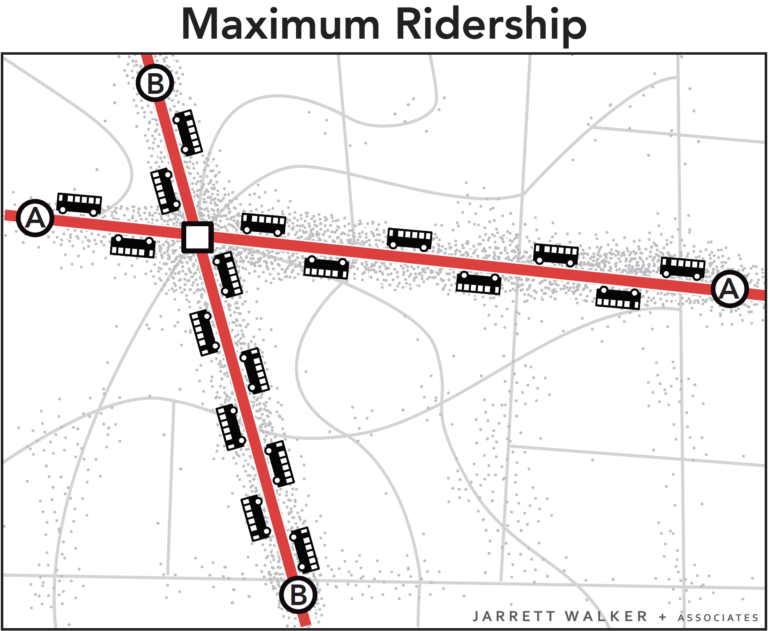
\includegraphics[width=\linewidth]{Presentation/diagrams/covVersusRide_2.png}
  \caption{Optimizing for Ridership \cite{walker2012}}\label{fig:ridership}
\endminipage\hfill
\minipage{0.49\textwidth}%
  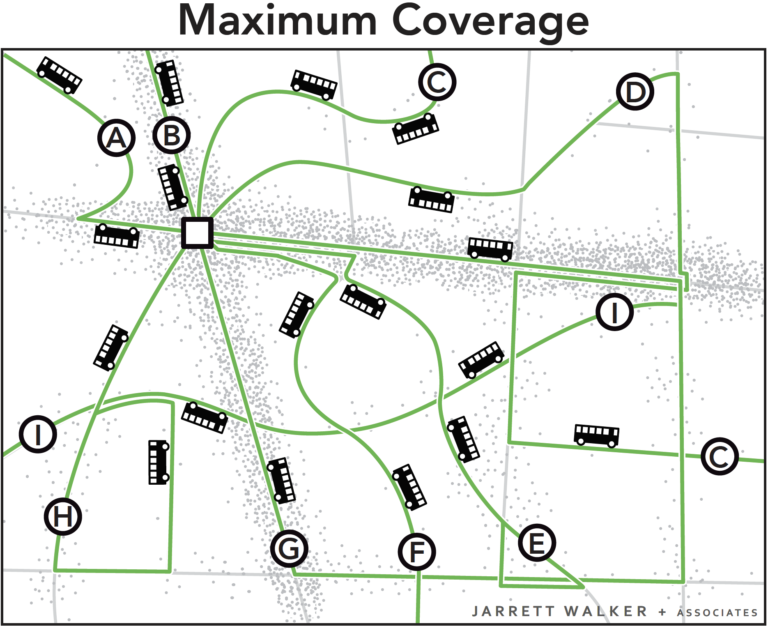
\includegraphics[width=\linewidth]{Presentation/diagrams/covVersusRide_3.png}
  \caption{Optimizing for Coverage \cite{walker2012}}\label{fig:coverage}
\endminipage
\end{figure}
\textbf{Other examples of trade-offs:}
\begin{enumerate}
    \item \textit{User Costs} versus \textit{Operator Costs}.  
    \item \textit{Network Simplicity} versus \textit{Functionality}. 
    \item \textit{Direct} versus \textit{Frequency}. 
\end{enumerate}
\end{frame}

\begin{frame}{Genetic Algorithms}
    \fbox{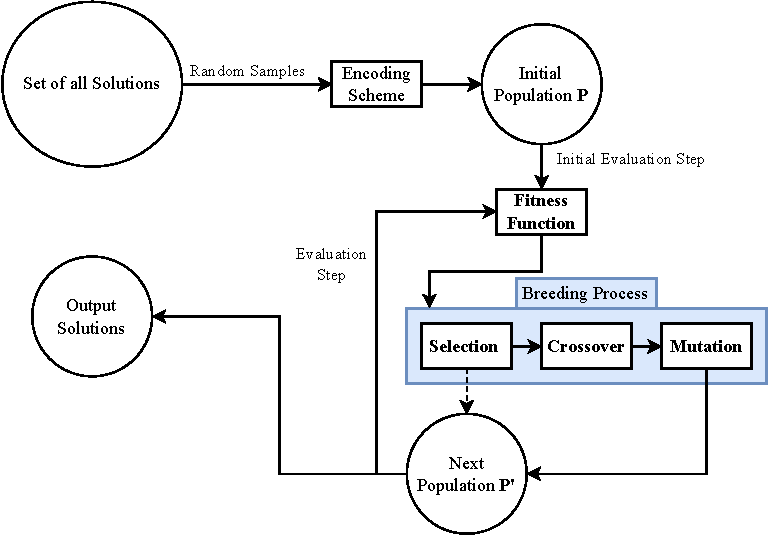
\includegraphics[width=\linewidth]{Presentation/diagrams/general_ga.pdf}}
\end{frame}

\begin{frame}{The Crossover Operation}
\begin{figure}
\minipage{0.49\textwidth}
  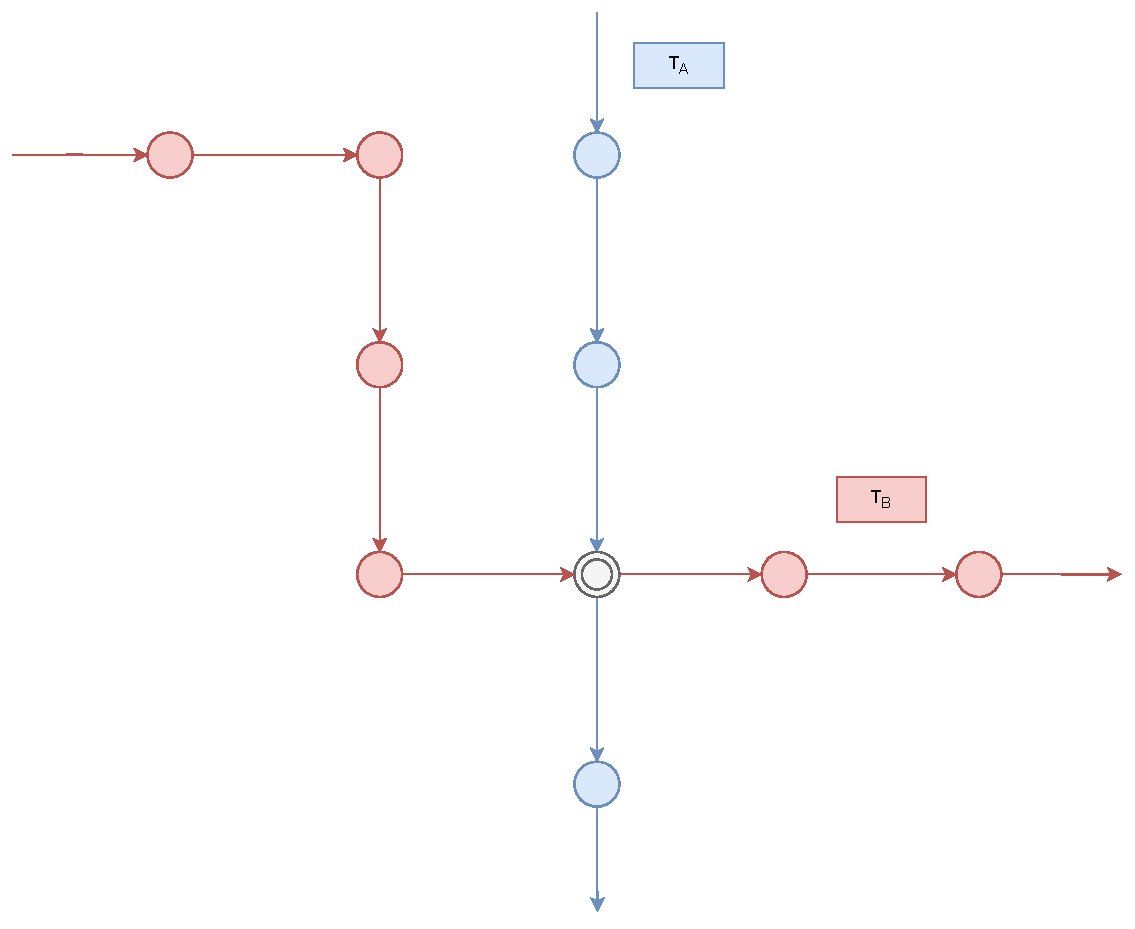
\includegraphics[width=\linewidth]{Presentation/diagrams/route-crossover1.pdf}
  \caption{Original 'parent' routes}\label{fig:parents}
\endminipage\hfill
\minipage{0.49\textwidth}%
  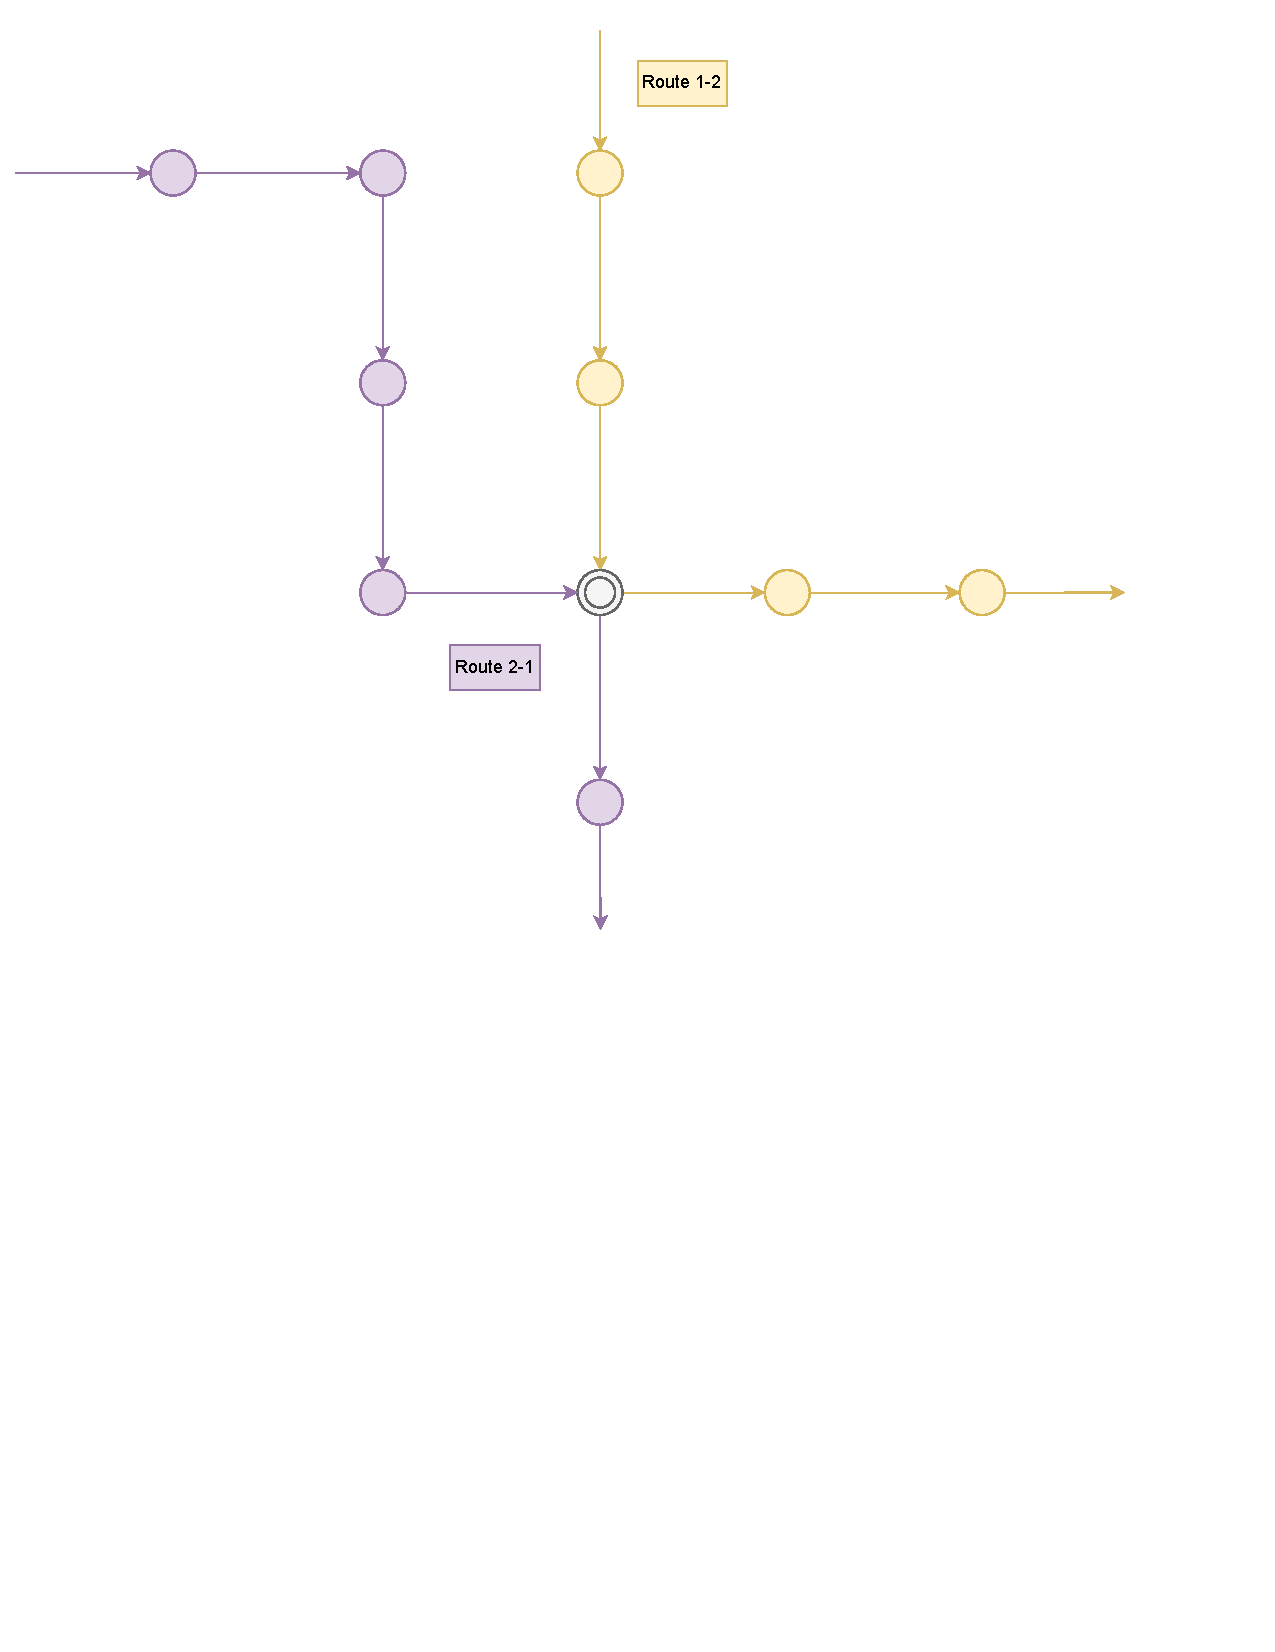
\includegraphics[width=\linewidth]{Presentation/diagrams/route-crossover2.pdf}
  \caption{New 'children' routes}\label{fig:children}
\endminipage
\begin{itemize}
    \item Focus on \textbf{transfer points} as crossover points. 
    \item Work with \textbf{simple routes} where only transfer points are considered. 
\end{itemize}
\end{figure}
\end{frame}


\begin{frame}{Next step: Processing Data}
    \fbox{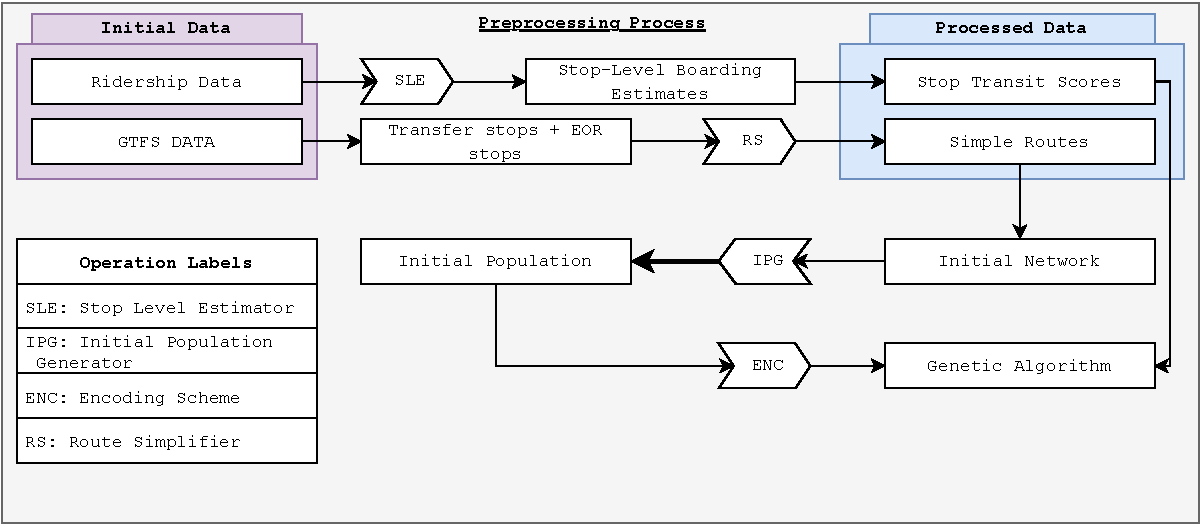
\includegraphics[width=\linewidth]{Presentation/diagrams/preprocessing_steps.pdf}}
    \begin{itemize}
        \item \textbf{Ridership Data:} Average total ridership by month by route. 
        \item \textbf{GTFS Data:} General Transit Feed Specification. 
    \end{itemize}
\end{frame}


\begin{frame}{Bibliography}
    \printbibliography
\end{frame}

\end{document}